\section{Cloud Native Anwendungen}
\label{sec:cloud-native-anwendungen}

% Was ist eine Cloud Native Anwendung?
% Merkmale
\subsection{Skalierbarkeit}
Von \textit{Cloud-native} Anwendungen wird unter anderem erwartet, dass diese schnell hoch skalieren können um einer steigenden Nutzerzahl gerecht zu werden \cite[Vgl.][S. 1ff]{Armbrust2009} \cite[Vgl.][S. 234]{Villamizar2017}. Um die Vorteile der Cloud aber auch hinsichtlich der Kosten nutzen zu können müssen die Services genauso herunter zu skalieren sein \cite[Vgl.][S. 884]{Adzic2017}.

Skalierbarkeit bedeutet in diesem Zusammenhang, dass die bereitgestellten IT-Ressourcen, wie Rechen- oder Speicherkapazität an die aktuelle Last angepasst werden können und entsprechen erhöht oder oder reduziert werden \cite[Vgl.][S. 15]{Reinheimer2018}\cite[Vgl.][]{Geißler2019}. Dabei wird in zwei Arten der Skalierung eines Systems unterschieden: \textbf{vertikale Skalierung} und \textbf{horizontale Skalierung} \cite[Vgl.][]{Geißler2019}\cite[Vgl.][]{VMware}

\begin{figure}[H]
    \centering
    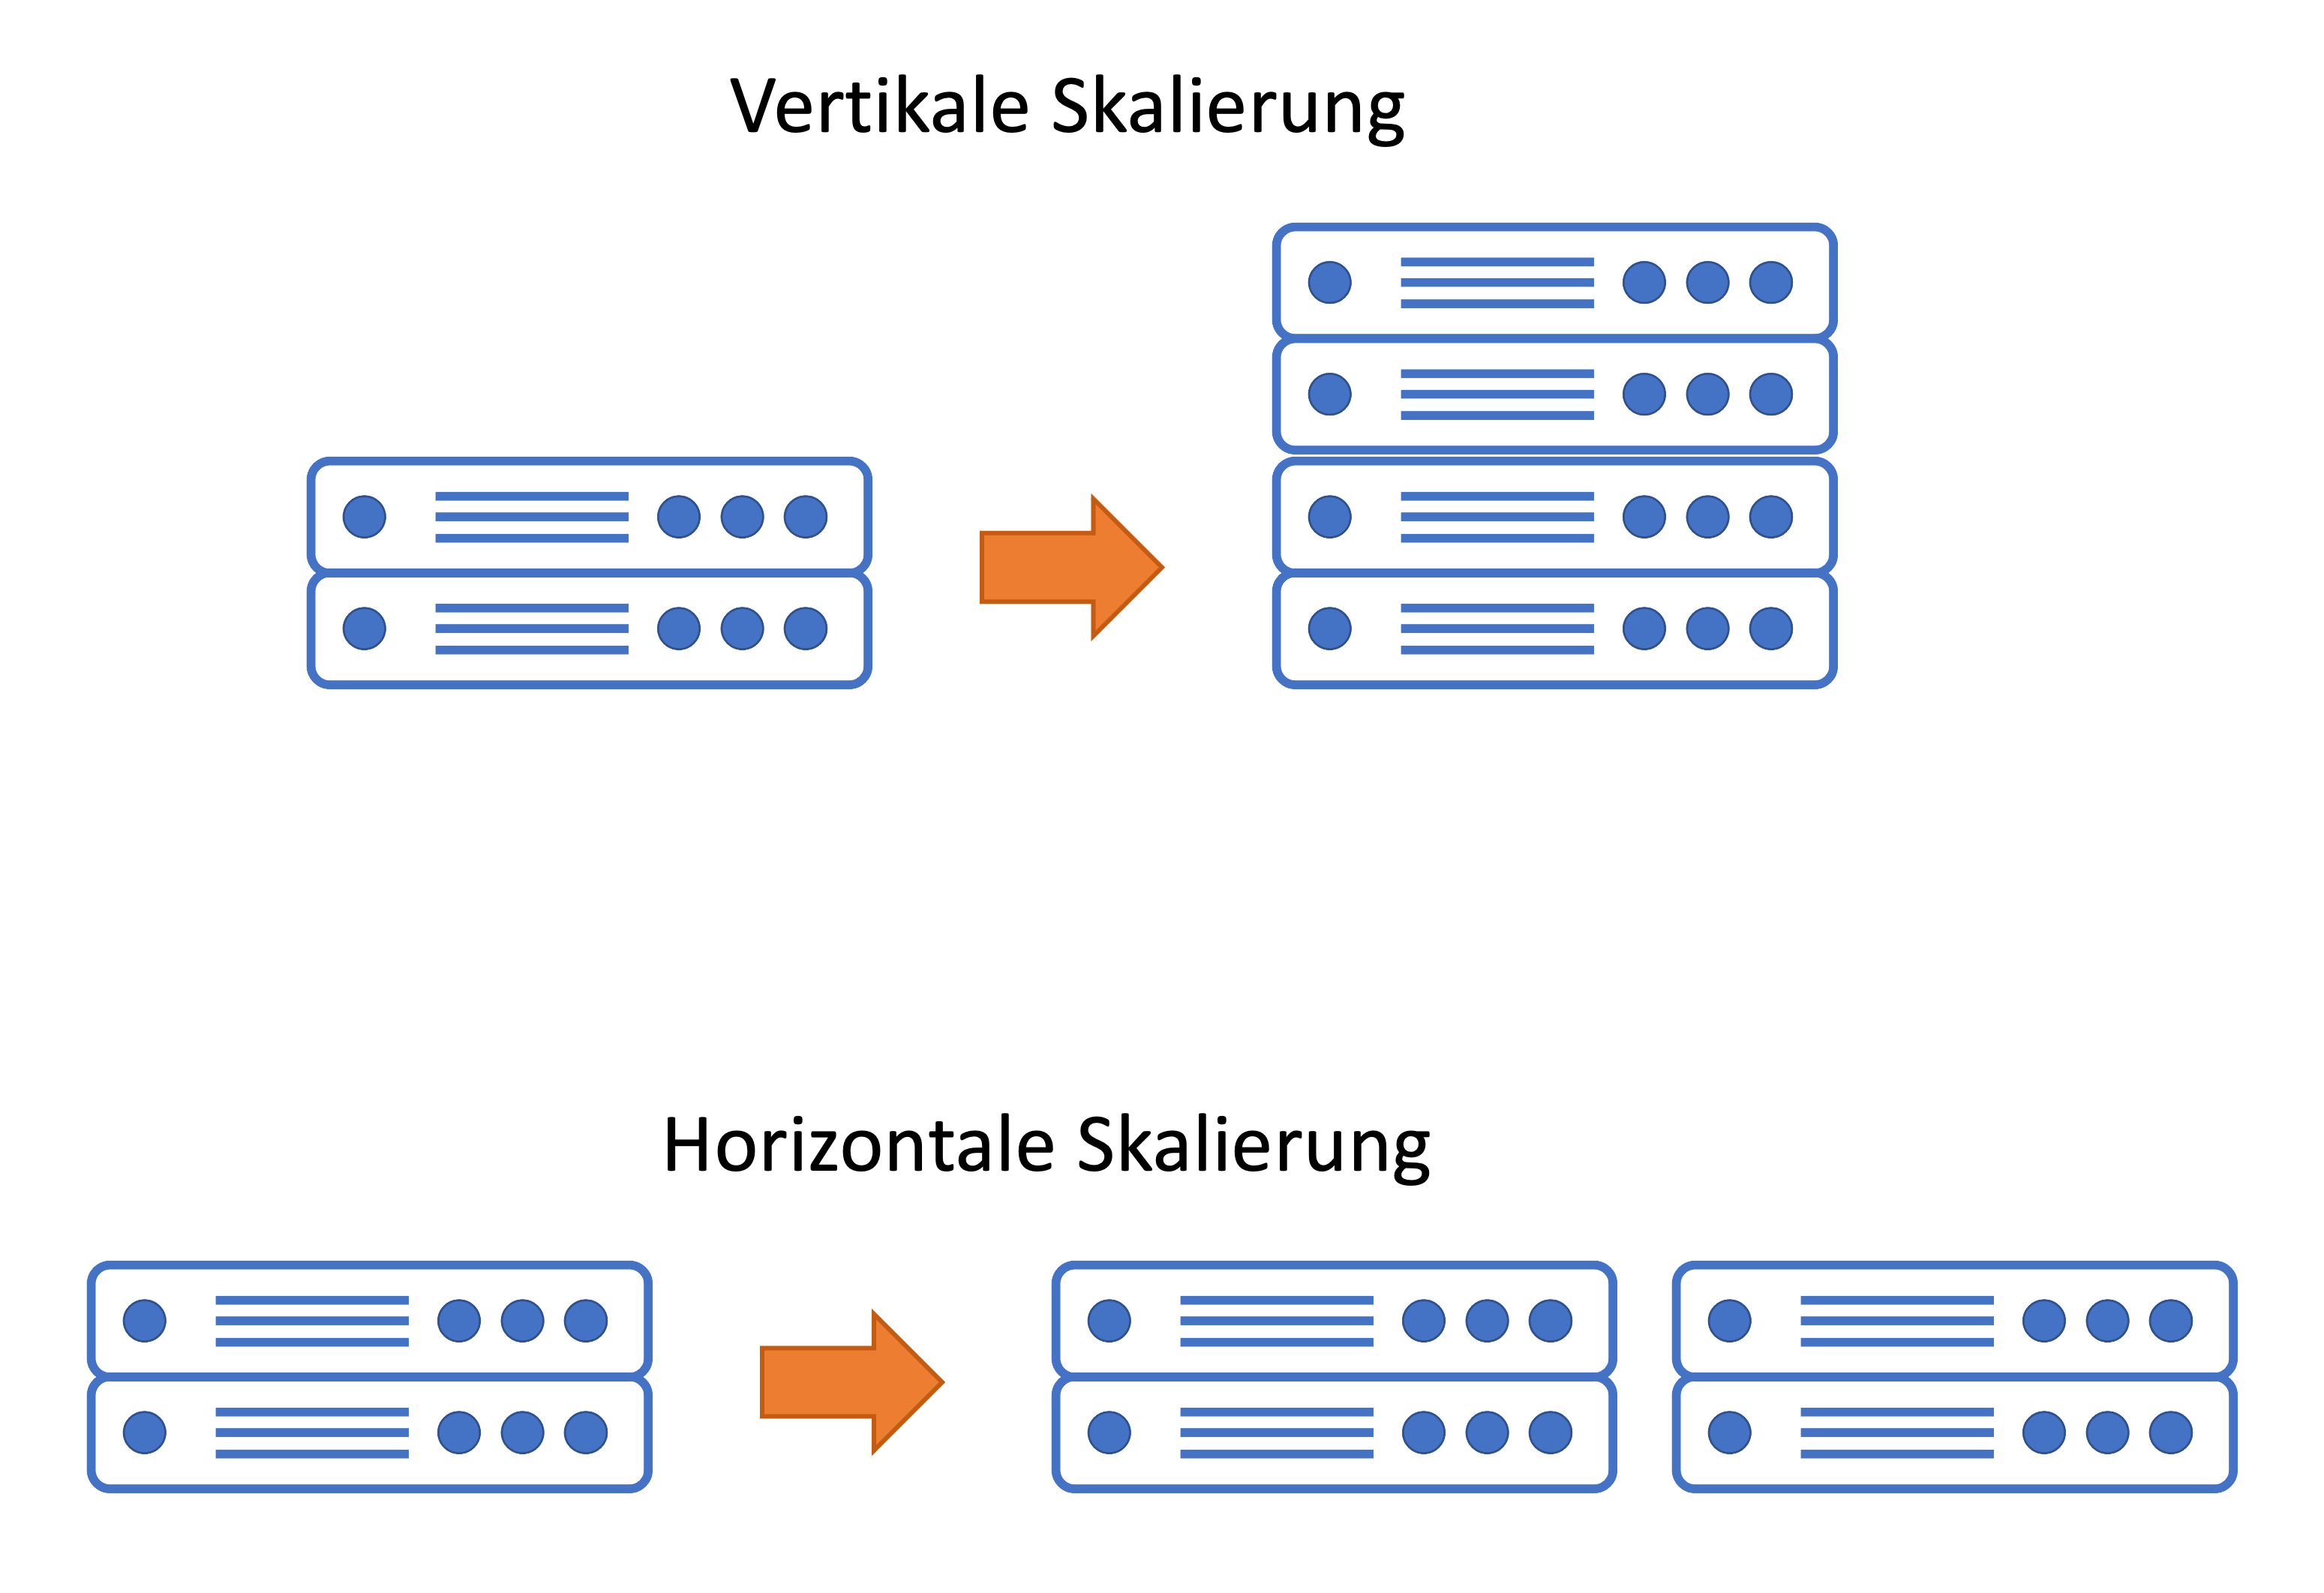
\includegraphics[width=0.65\textwidth]{scale-up_scale-out.png}
    \caption{Vertikale vs. Horizontale Skalierung \cite[Nachbildung nach][]{Bachmann2019}}
    \label{fig:scale-up-scale-out}
\end{figure}

\textbf{Vertikale Skalierung:}
Bei der vertikalen Skalierung wird zu einer Einheit innerhalb eines Systems zusätzliche Rechenleistung oder zusätzlicher Speicher hinzugefügt. Diese Art der Skalierung wird auch als \glqq{Scale-up}\grqq{} bezeichnet, abgeleitet von dem Erhöhen der Leistung. Die vertikale Skalierung ist jedoch dadurch limitiert, dass bei der Leistungsaufstockung hardwareseitig Grenzen gesetzt sind \cite[Vgl.][]{Geißler2019}\cite[Vgl.][]{VMware}. \pagebreak

\textbf{Horizontale Skalierung:}
Zur horizontalen Skalierung werden dagegen nicht die Ressourcen innerhalb einer Einheit erhöht, sondern weitere Einheiten beziehungsweise Knoten zu einem System hinzugefügt. Die Aufgaben werden dann auf mehreren Systemen durchgeführt, oder zum Beispiel eine Anwendung in mehreren Containern parallel ausgeführt. Horizontale Skalierung wird auch als \glqq{Scale-out}\grqq{} bezeichnet, da ein System hier in seiner Breite erweitert wird. In der Theorie sind der horizontalen Skalierung keine Grenzen gesetzt \cite[Vgl.][]{Geißler2019}\cite[Vgl.][]{VMware}.

\subsection{Fehlertoleranz}
Eine weitere Anforderung an Cloud-native Anwendungen ist die Fehlertoleranz. Es sollte grundsätzlich davon ausgegangen, dass Fehler auftreten können und diese abgefangen werden müssen \cite[Vgl.][S. 17]{Gannon2017}. Zu diesen Fehlern gehört unter anderem das Abstürzen von Container und Hardware- oder Netzwerkfehler.

\subsection{Schnelle Bereitstellung}
\dots
\pagebreak